\documentclass[tikz, border=8pt]{standalone}
\usepackage[T1]{fontenc}
\usepackage{tgpagella}
\usepackage{mathpazo}
\usepackage{tikz}
\usepackage{amsmath}
\usepackage{xcolor}
\usepackage{fontawesome5}
\usetikzlibrary{arrows.meta, shapes.geometric, calc}

\definecolor{cAudio}{HTML}{F5EFE3}
\definecolor{cEnc}{HTML}{DDE9EC}
\definecolor{cEncB}{HTML}{2D8294}
\definecolor{cAdp}{HTML}{F0DFC9}
\definecolor{cAdpB}{HTML}{B07849}
\definecolor{cLLM}{HTML}{F4E6D5}
\definecolor{cLLMB}{HTML}{A0763C}
\definecolor{cPrompt}{HTML}{F1ECE3}
\definecolor{cPromptB}{HTML}{8E7A55}
\definecolor{cTok}{HTML}{E5EEF0}
\definecolor{cTokB}{HTML}{5E8090}
\definecolor{cBound}{HTML}{ECDFD3}
\definecolor{cBoundB}{HTML}{9C7558}
\definecolor{cAuT}{HTML}{F6E1CF}
\definecolor{cAuTB}{HTML}{C77F45}
% token-cell modality colours (high cool/warm contrast)
\definecolor{cAudC}{HTML}{BCDBE2}
\definecolor{cAudCB}{HTML}{2D8294}
\definecolor{cTxtC}{HTML}{F3DFA6}
\definecolor{cTxtCB}{HTML}{C0952F}

\newcommand{\frozenIcon}{\textcolor{cEncB}{\faSnowflake}}
\newcommand{\fireIcon}{\textcolor{cLLMB!90!red}{\faFire}}

\newcommand{\WaveformPictogram}{%
  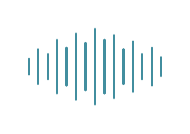
\begin{tikzpicture}[baseline=-0.6ex]
    \foreach \i/\h in {%
        0/0.10, 1/0.22, 2/0.16, 3/0.34, 4/0.24,
        5/0.42, 6/0.30, 7/0.48, 8/0.34, 9/0.40,
        10/0.22, 11/0.32, 12/0.16, 13/0.24, 14/0.12%
    }{
      \pgfmathsetmacro{\xpos}{-0.84 + \i*0.12}
      \draw[line width=0.85pt, line cap=round, draw=cEncB!90]
        (\xpos, -\h) -- (\xpos, \h);
    }
  \end{tikzpicture}%
}

\tikzset{
  module/.style    ={draw, rounded corners=3pt, align=center,
                     font=\small, line width=0.7pt,
                     minimum height=0.88cm},
  encoder/.style   ={module, fill=cAuT, draw=cAuTB, minimum width=3.2cm},
  promptbox/.style ={module, fill=cPrompt, draw=cPromptB, minimum width=3.0cm},
  biasbox/.style   ={module, fill=cAdp!55, draw=cAdpB, minimum width=3.1cm},
  tokenizer/.style ={module, fill=cTok, draw=cTokB, minimum width=3.2cm},
  ragbox/.style    ={module, fill=cBound, draw=cBoundB, minimum width=2.7cm},
  hpool/.style     ={draw=cAdpB, fill=cAdp, line width=0.75pt,
                     cylinder, shape border rotate=90, aspect=0.22,
                     minimum width=2.2cm, minimum height=1.75cm,
                     align=center, font=\small},
  llmbox/.style    ={module, fill=cLLM, draw=cLLMB, line width=0.85pt,
                     minimum width=11.8cm, minimum height=0.92cm,
                     font=\normalsize},
  outbox/.style    ={module, fill=white, draw=black!50, font=\small,
                     minimum width=2.2cm},
  tokcell/.style   ={draw, line width=0.4pt, minimum width=0.40cm,
                     minimum height=0.40cm, inner sep=0pt},
  cellText/.style  ={tokcell, fill=cTxtC, draw=cTxtCB},
  cellAudio/.style ={tokcell, fill=cAudC, draw=cAudCB},
  flow/.style      ={-Stealth, line width=0.7pt, draw=black!70},
  dashedflow/.style={flow, dashed, draw=black!55},
  edgelabel/.style ={font=\scriptsize, text=black!55,
                     fill=white, inner sep=1pt},
  legendtxt/.style ={font=\scriptsize, text=black!75},
  mergepoint/.style={circle, fill=black!60, inner sep=1.1pt}
}

\begin{document}
% Grid layout (cm): three well-separated columns feeding a shared
% sequence / LLM spine. Every connector is orthogonal (straight or
% right-angle folds) and routed through the gaps between modules so
% that no line overlaps a box.
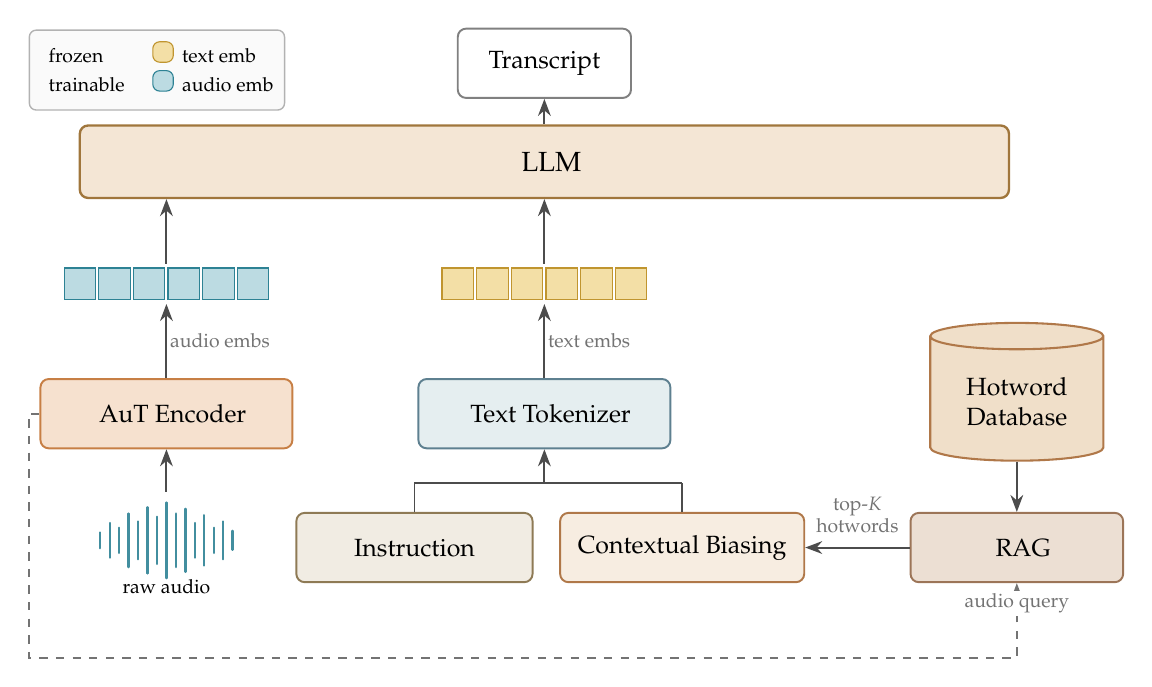
\begin{tikzpicture}

  % ===== spine (x = 0) =================================================
  \node[outbox] (out) at (0, 6.35) {Transcript};
  \node[llmbox] (llm) at (0, 5.10) {%
    \fireIcon~~LLM%
  };
  \node[draw=none, minimum width=12cm, minimum height=0.5cm]
        (seqbox) at (0, 3.55) {};

  % audio-embedding cells (left group, above the AuT column)
  \foreach \i in {0,1,2,3,4,5}{
    \pgfmathsetmacro{\xc}{-4.8 + (\i-2.5)*0.44}
    \node[cellAudio] at (\xc, 3.55) {};
  }
  % text-embedding cells (centre group, above the tokenizer column)
  \foreach \i in {0,1,2,3,4,5}{
    \pgfmathsetmacro{\xc}{0 + (\i-2.5)*0.44}
    \node[cellText] at (\xc, 3.55) {};
  }

  \draw[flow] (llm.north)    -- (out.south);
  \draw[flow] (seqbox.north) -- (llm.south);
  \draw[flow] ([xshift=-4.8cm]seqbox.north) -- ([xshift=-4.8cm]llm.south);

  % ===== left column: audio (x = -4.8) =================================
  \node[encoder] (aut)  at (-4.8, 1.90) {\fireIcon~~AuT Encoder};
  \node[draw=none, font=\small, align=center] (wave) at (-4.8, 0.20) {%
    \WaveformPictogram\\[-1pt]\scriptsize raw audio%
  };
  \draw[flow] (wave.north) -- (aut.south);
  \draw[flow] (aut.north) -- (aut.north |- seqbox.south)
        node[midway, edgelabel, right] {audio embs};

  % ===== centre column: text (x = 0) ===================================
  \node[tokenizer] (tok) at (0, 1.90) {\frozenIcon~~Text Tokenizer};
  \draw[flow] (tok.north) -- (tok.north |- seqbox.south)
        node[midway, edgelabel, right] {text embs};

  \node[promptbox] (instr) at (-1.65, 0.20) {Instruction};
  \node[biasbox]   (bias)  at ( 1.75, 0.20) {Contextual Biasing};
  % fork: the two prompt sources join a horizontal bar that forks into
  % branches; only the trunk into the tokenizer carries an arrowhead.
  \draw[line width=0.7pt, draw=black!70] (instr.north) -- (-1.65, 1.02);
  \draw[line width=0.7pt, draw=black!70] (bias.north)  -- ( 1.75, 1.02);
  \draw[line width=0.7pt, draw=black!70] (-1.65, 1.02) -- ( 1.75, 1.02);
  \draw[flow] (0, 1.02) -- (tok.south);

  % ===== right column: RAG (x = 6.0) ===================================
  \node[hpool]  (hpool) at (6.00, 2.05) {Hotword\\Database};
  \node[ragbox] (rag)   at (6.00, 0.20) {\fireIcon~~RAG};
  \draw[flow] (hpool.south) -- (rag.north);
  \draw[flow] (rag.west) -- (bias.east)
        node[midway, edgelabel, above=4pt, align=center] {top-$K$\\hotwords};

  % ===== audio query: dashed orthogonal bus below every module =========
  \coordinate (aqA) at (-6.55, 1.90);
  \coordinate (aqB) at (-6.55, -1.20);
  \coordinate (aqC) at ( 6.00, -1.20);
  \draw[dashedflow] (aut.west) -- (aqA) -- (aqB) -- (aqC) -- (rag.south)
        node[pos=0.55, edgelabel, above] {audio query};

  % ===== legend (top-left corner, compact) =============================
  \node[draw=black!30, rounded corners=2.5pt, fill=black!2,
        line width=0.5pt, anchor=north west, align=left, inner sep=4pt]
        at (-6.55, 6.78) {%
    \scriptsize
    \renewcommand{\arraystretch}{1.1}%
    \begin{tabular}{@{}c@{\hspace{3pt}}l@{\hspace{10pt}}c@{\hspace{3pt}}l@{}}
      \frozenIcon & frozen &
      \tikz\node[cellText,  minimum width=0.26cm, minimum height=0.26cm]{}; & text emb\\
      \fireIcon   & trainable &
      \tikz\node[cellAudio, minimum width=0.26cm, minimum height=0.26cm]{}; & audio emb\\
    \end{tabular}%
  };

\end{tikzpicture}
\end{document}
